\documentclass[a4paper, dvipdfmx]{jsarticle}
\usepackage{amsmath,amssymb}
\usepackage[version=3]{mhchem}
\usepackage{booktabs}
\usepackage[dvipdfmx]{graphicx}
\usepackage{pdfpages}
\usepackage{siunitx}
\usepackage{url}
\usepackage{listings}
\usepackage{float}
\usepackage{longtable}

\title{科学と情報\\ 学期末レポート\\ SNS上の陰謀論的なテキストについての品詞に着目した考察}
\author{1年 \ \ C0TB5058  \ \ 高橋隆造   }
\begin{document}
\maketitle
\newpage
\section{はじめに}
今日、インターネットの発展により何らかの知識をインターネット上のウェブサイトから仕入れることが常態化している。しかしながら、インターネット上の知識は必ずしも正しいわけではなく、そのためインターネットを通して何らかの分野の知識を得るためには事前にその分野に関してある程度の知見があることが望ましい。しかしながら、実際にあらゆる分野でそれを満たすのは困難である。それどころか、近年は主にSNSや個人ブログにおいて、陰謀論と言われる非科学的な言説が蔓延している。この陰謀論は、反ワクチン運動などと結びつくことによりそれを信じる者及びその周りにいる人々に害を及ぼすという点で、従来のいわゆる都市伝説と区別できると考えられる。今回のレポートでは特にtwitter上の陰謀論的な言説について定量的な分析を行うとともに、陰謀論的な言説とそうでないものの定量的な区別を試みる。
\section{Twitter上での陰謀論的な言説と非陰謀論的な言説の抽出}
今回、分析を行うに当たり、SNSプラットフォーム「Twitter」上から陰謀論的な言説と思われるものと、そうでないより一般的な言説と思われる二種類のテキストを抽出し、分析した。2種類のテキストを抽出するに当たり、特に今般の情勢からつぶやかれることの多いコロナウイルスについてのキーワードのうち、陰謀論的と思われるキーワードとより一般的なキーワードをそれぞれ4種類ずつ用意した。各キーワードを以下の表にあらわす。
\begin{table}[ht]
\centering
\begin{tabular}{rr}
陰謀論的なキーワード & 一般的なキーワード \\
 \hline
ワクチン AND 2回目 & ワクチン AND 人口削減 \\
医療崩壊 & コロナ AND 茶番 \\
医療 & 枠珍 \\
ワクチン & コロナ脳 \\
  \hline
\end{tabular}
\end{table}
なお、ここで上げたキーワードはすべて著者が実際に見聞きした者に限られるため、著者のバイアスが多分に含まれている可能性があることには留意したい。
\par
これらキーワードを含むツイートをそれぞれ22個づつtwitter api\cite{s1}を用いて集めた。
\section{2つのキーワード群での品詞の使われ方についての分析}
ここで、それぞれのキーワードを含む分がどのような品詞の構成を持っているかに注目した。陰謀論的なキーワードを含んだテキストのグループと、一般的なキーワードを含んだテキストのグループのそれぞれを構成する品詞を取り出し、名詞、動詞、形容詞、副詞、助詞、接続詞、助動詞、連体詞、感動詞、その他の品詞に分解し、それぞれ集計した。まず、それぞれのグループでどの品詞が一つのツイートの中で使われる頻度の平均を求めたものを以下の図に示す。これは、各ツイートについて、任意の品詞の使用回数をそのツイートの全品詞数で割ったものの平均を表している。
\begin{figure}[H]
\begin{center}
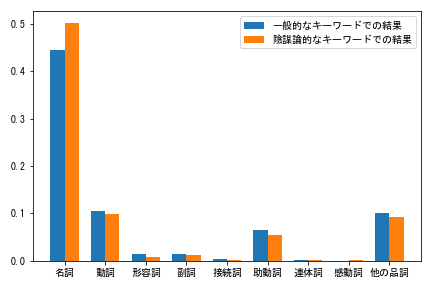
\includegraphics[width=100mm]{../images/fig3.png}
\caption{それぞれに使われている品詞の頻度の平均}
\end{center}
\end{figure}
ここで、差が最も顕著なのが名詞の使用である。名詞の使用は陰謀論的なキーワードを含むテキストのグループが一般的なキーワードを含むテキストのグループより優越している。次に、名詞に着目して分析を行う。
\subsection{名詞の使われ方についての詳細}
両グループの名詞の使用頻度について、前述した方法で使用頻度を算出したときの使用頻度の分布について、それぞれのグループごとに表したヒストグラムを以下に表示する。
\begin{figure}[H]
\begin{center}
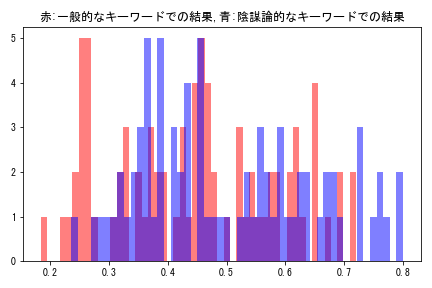
\includegraphics[width=100mm]{../images/fig4.png}
\caption{それぞれに使われている品詞の頻度の平均}
\end{center}
\end{figure}
ここで、2グループ間の平均値の差は0.5である。分散は陰謀論的なキーワードを含むテキストのグループの方が大きく、それぞれ0.021と0.019だった。
また、対応なしt検定を行った。このときp値は0.026となり、有意差がないという帰無仮説は棄却された。つまり、一般的なキーワードを含むテキストのグループと陰謀論的なキーワードを含むテキストのグループの間での名詞の登場頻度には有意差があるといえる。
\section{結論}
以上より、一般的なキーワードを含むテキストのグループと陰謀論的なキーワードを含むテキストのグループにおいて、前者の方が名詞を多く含むことがわかった。何故陰謀論的なキーワードを含むテキストで名詞の頻度が多くなるかについては、追加の調査が必要である。
\par
しかしながら、その差は小さく、これが陰謀論的な言説を見分ける容易な方法であるとは言いがたい。
\begin{thebibliography}{10}
  \bibitem{s1} twitter api \url{https://help.twitter.com/ja/rules-and-policies/twitter-api} 2021/08/03日閲覧
\end{thebibliography}
\end{document}
